%
\documentclass[
    fontsize=12pt,
    paper=a4,
    pagesize=auto,
    parskip=false,
    titlepage=on,
    english
]{scrartcl}
\usepackage[utf8]{inputenc}
\usepackage[T1]{fontenc}
\usepackage{babel}
\usepackage{amsmath}
\usepackage{lmodern}
\usepackage{amssymb}

\usepackage{graphicx}
\usepackage{siunitx}
\usepackage{microtype}
\usepackage{float}
\usepackage{commath}
\usepackage{hyperref}

\usepackage{tikz}
\usepackage{caption}
\usepackage{subcaption}

\newcommand{\inlinecode}{\texttt}


\title{Interactive Exploration of Cosmological Dark Matter Simulation Data}
\subtitle{Instruction Manual}
\author{Voreen Team ((TODO: alternativ?))}

\begin{document}

\maketitle

\newpage
\tableofcontents

\newpage

\section{Data}
\label{sec:data}
Example data can be obtained from the official contest homepage~\cite{contesthp}.
After downloading extract the archive to a location of your choice (later referred to as \$ARCHIVE\_ROOT).
Our application makes use of two types of data provided: Single dark matter particle data and halo structures.
Particle data resides in multiple files in folder \inlinecode{\$PARCILE\_FOLDER:=\$ARCHIVE\_ROOT/ds14\_scivis\_0128/}.
Halo data resides in multiple files in folder \inlinecode{\$HALO\_FOLDER:=\$ARCHIVE\_ROOT/ds14\_scivis\_0128/rockstar/hlists/}.

\section{Building}
For basic build instructions refer to the voreen build instructions at~\cite{voreen-build}.
Additionally, make sure to set the CMake variable \inlinecode{VRN\_MODULE\_VISCONTEST2015} to \inlinecode{ON}.
This application additionally makes use of the HDF5 library~\cite{hdf5lib} to store data sets.
If you are running a unix-like operating system, please make sure to have an up to date version of libhdf5 (tested with version 1.8) installed.
The windows version of our application is bundled with a hdf5 library, so no additional steps need to be taken.

\section{Starting the Application}
\label{sec:start}
After successfully building the application you should find the executable in the bin subfolder of the build location. ((TODO: stimmt das?))
Execute it to be able to open the main window of our application.
The window is devided into two panes:
The right pane (configuration pane) can be used to configure parameters of the application.
It is devided into seven sections (Input Data, Volume, Particles (global), Particle Time Animation, Halos, Particles (local), and General Settings).
The larger left pane is used to render the visualizations of the dark matter data.
It presents four views in different tabs which are described in more detail in section~\ref{sec:interaction}


In order to explore the dark matter data you must first supply the application with paths to the halo and particle data obained as described in section~\ref{sec:data}.
To do so, first expand the section ``Input Data'' and then click on ``Load Halos'' and ``Load Particles'' (highlighted blue in Figure~\ref{fig:loadinstructions}) and navigate and select \inlinecode{\$PARTICLE\_FOLDER} and \inlinecode{\$HALO\_FOLDER}, respectively.
\begin{figure}[h]
    \label{fig:loadinstructions}
    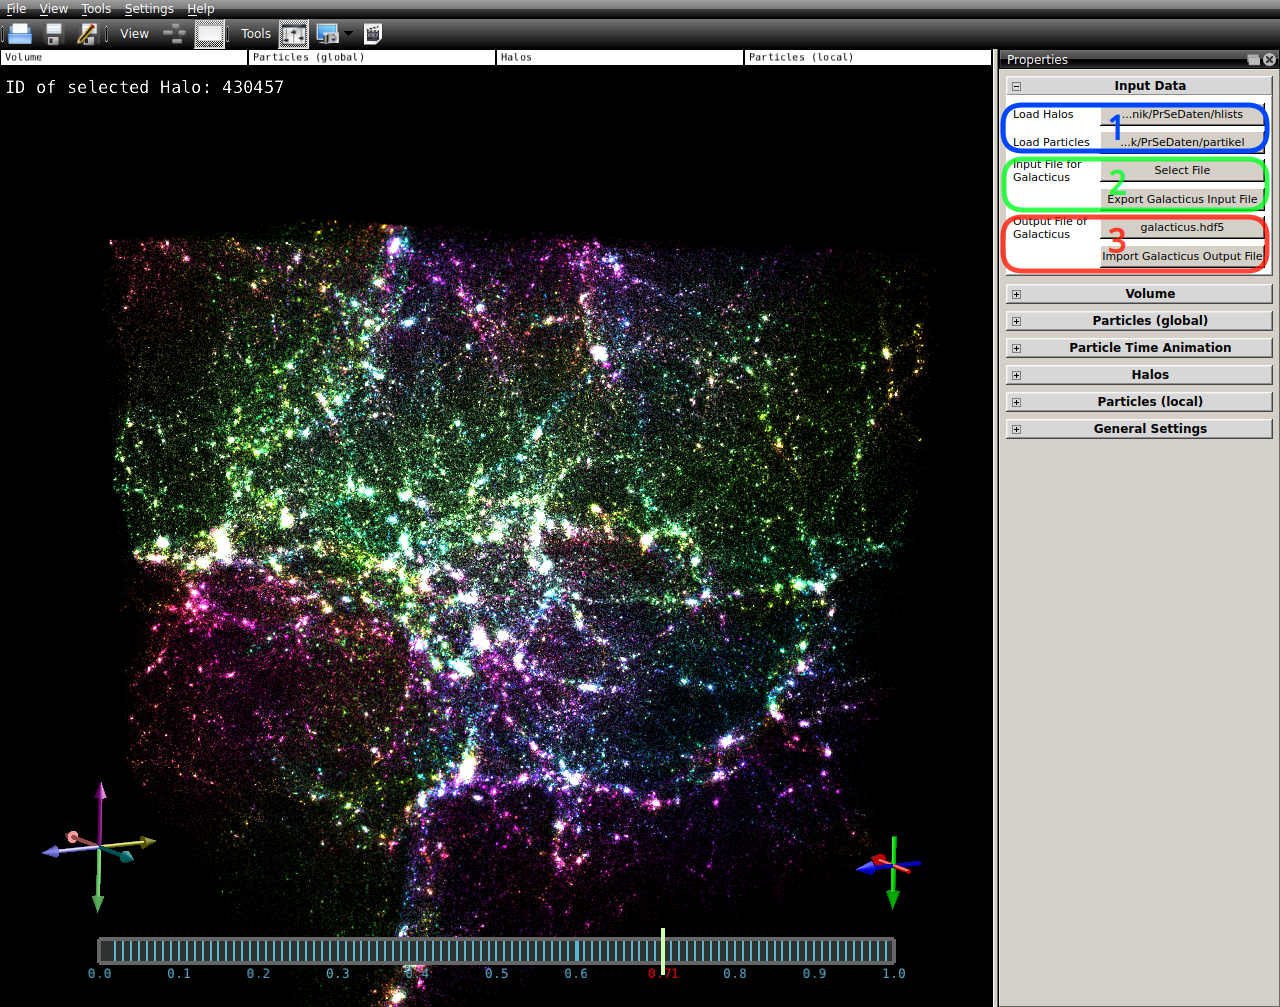
\includegraphics[width=1.0\textwidth]{images/loadinstructions.png}
        \caption{Importing/Exporting Data: 1. Import Halo/Particle Data. 2. Export Data to Galacticus. 3. Import Data from Galacticus}
\end{figure}
When loading for the first time, the halo files have to be parsed and converted to an internal binary format which may take some time.
However, the result is cached and does not need to be recomputed when starting the application a second time.

\section{Galacticus}
\label{sec:galacticus}
Our application makes use of six of the properties of halos provided by the files in \inlinecode{\$HALO\_FOLDER}: Position, velocity, angular momenta, radius, mass and spin.
However, we provide means to interface with galacticus~\cite{galacticus} and add many more data columns to the provided halo data which, which can also be visualized using our application.
The first step is to export the currently loaded halo data (see section~\ref{sec:start}) to a galacticus compatible format.
To do so, choose a file name (\inlinecode{:=\$GALACTICUS\_INPUT}) as the ''Input File for Galacticus'', e.g. \inlinecode{voreen\_halo\_output.xml}.
As a second step you may now run galacticus: Navigate into the Galacticus source folder that contains the executable \inlinecode{Galacticus\_v0.9.4\_latest\_x86\_64.exe} (or similar).
Then run the executable and supply the voreen generated XML-file as the first and only command line argument: \inlinecode{./Galacticus\_v0.9.4\_latest\_x86\_64.exe \$GALACTICUS\_INPUT}.
When finished, Galacticus should have generated a filename called ((TODO)) (\inlinecode{:=\$GALACTICUS\_OUTPUT}).
Finally return to the application window and select \inlinecode{\$GALACTICUS\_OUTPUT} as the ''Output File of Galacticus''.
Now click ''Import Galacticus Output File'' to finish the Galacticus data import.

\section{Interaction}
\label{sec:interaction}
\subsection{General Interaction}
When not mentioned otherwise, the camera is positioned and controlled via the trackball metaphora.
The camera is focused on the current object of interest.
The orientation of the camera can be changed by moving the cursor while simultaniously holding down the left mouse button.
The distance of the camera to the object of interest can be manipulated by scrolling.
Moving the cursor while holding the shift and left mouse button will move the focus of the camera in the plane of the canvas.

\subsection{Views}
\subsubsection{Volume}
The ``Volume'' tab visualizes the special distribution of particles.
It is divided into four subpanes.
The top left subpane shows a 3D rendering of the volume.
The trackball center is initially positioned in the center of the volume.
The other three subpanes show 2D renderings of slices of the volume in the x-, y-, and z-dimension
Scrolling sliceview-pane moves the slice in the direction perpendicular to the slice within the volume.
Scrolling while pressing the CTRL-Button will zoom in or out.
The focus of the camera can be shifted by holding down CTRL and the left mouse button and moving the cursor.
Parameters for this view can be changed in the ``Volume'' section of the configuration pane.
Subpanes of views can be temporarily expanded by doubleclicking within them.
Perform another doubleclick to return to the original view.

\subsubsection{Particles (global)}
In the ``Particles (global)'' tab all particles are individually rendered using sprites.
As in the 3D volume view the trackball position is initialized in the center of the universe cube.
In the configuration pane the sections ``Particles (global)'' and ``Particle Time Animation'' refer to this tab.
``Particle Time Animation'' can be used to animate the currently displayed time step.

\subsubsection{Halos}
The third tab, ``Halos'' shows three interactive subpanes.
The top right and bottom right pane show renderings of the halos in the current time step in their spacial position in the universe.
In these subpanes the trackball center is always set and moved to the position of the currently selected halo.
The top left subview visualizes the evolution of the currently selected halo in as a 2D merger tree visualization.
Halos in all three views can be selected and focused by clicking on the using the left mouse button.
General information about the currently selected halo and global halo properties can be found in the bottom left view.
The corresponding ``Halos'' section in the configuration pane can be expanded to change parameters used for the visualization.

\subsubsection{Particles (local)}
The fourth view ``Particles (local)'' can be used to track the local movement of dark matter particles comprising a halo.
The top right view again shows the currently selected halo and its neighbors positioned in the universe and can be used to navigate by clicking on other halos.
In this view this will not change the current halo selection.
Instead, all particles within the radius of the previously selected halo are rendered in the remaining three subviews.
The bottom two subviews render each particle indidually using sprites (left) or arrows (right) indicating their direction of movement.
The slider at the bottom can be used to change the currently displayed time step, which will affect the halo and the bottom two subviews.
If ``Follow Halo'' in the ``Particles (local)'' section of the configuration pane is activated, the camera will follow the halo focused in the top right subpane.
This is useful for tracking the movement of subhalos (and its particles) within the currently selected large halo.
If not activated, the camera will remain stationary when changing timesteps.
The top left subpane remains unaffected by a changed time step as it tracks the movement of individual particles over time.

For a general overview of functionality you may also watch our presentation video as submitted to the contest committee~\cite{contestvid}.

\begin{thebibliography}{9}
    \bibitem{voreen} Voreen (\url{http://voreen.uni-muenster.de/})
    \bibitem{contesthp} SciVis Contest 2015 (\url{http://darksky.slac.stanford.edu/scivis2015/data/ds14_scivis_0128.tar})
    \bibitem{voreen-build} Voreen build instructions (\url{http://www.uni-muenster.de/Voreen/documentation/build_instructions.html})
    \bibitem{hdf5lib} HDF5 library (\url{https://www.hdfgroup.org/})
    \bibitem{galacticus} Galacticus (\url{http://voreen.uni-muenster.de://sites.google.com/site/galacticusmodel/})
    \bibitem{contestvid} Contest submission video (\url{http://viscg.uni-muenster.de/publications/2015/SBDVRSFH15/muenster_as_tb.mp4})
\end{thebibliography}



\end{document}

